\documentclass[a4paper,10pt,usenames]{article}
%\documentclass[color=pdftex]{beamer}
\usepackage[T2A]{fontenc}
\usepackage[utf8x]{inputenc}
\usepackage{ucs}
\usepackage{cmap}
\usepackage[english,russian]{babel}
\usepackage{amsmath}
\usepackage{graphicx}
\usepackage{indentfirst}
\usepackage{ucs} 
\usepackage[utf8x]{inputenc}
\usepackage{caption}
\usepackage{placeins}
\usepackage{listings}
\usepackage{hyperref}
\usepackage[usenames,dvipsnames]{color}    
\lstset{ 
  language=R,                     % the language of the code
  basicstyle=\small\ttfamily, % the size of the fonts that are used for the code
  numbers=left,                   % where to put the line-numbers
  numberstyle=\small\color{Blue},  % the style that is used for the line-numbers
  stepnumber=1,                   % the step between two line-numbers. If it's 1, each line
                                  % will be numbered
  numbersep=5pt,                  % how far the line-numbers are from the code
  backgroundcolor=\color{white},  % choose the background color. You must add \usepackage{color}
  showspaces=false,               % show spaces adding particular underscores
  showstringspaces=false,         % underline spaces within strings
  showtabs=false,                 % show tabs within strings adding particular underscores
  frame=single,                   % adds a frame around the code
  rulecolor=\color{black},        % if not set, the frame-color may be changed on line-breaks within not-black text (e.g. commens (green here))
  tabsize=2,                      % sets default tabsize to 2 spaces
  captionpos=b,                   % sets the caption-position to bottom
  breaklines=true,                % sets automatic line breaking
  breakatwhitespace=false,        % sets if automatic breaks should only happen at whitespace
  keywordstyle=\color{RoyalBlue},      % keyword style
  commentstyle=\color{YellowGreen},   % comment style
  stringstyle=\color{ForestGreen}      % string literal style
} 


\title{Исследование спайкового кода}
\author{Чернышев Алексей}
\setlength{\parindent}{1cm}
\def\la{\left\langle\rule{0pt}{3em}}
\def\ra{\right\rangle}
\newcommand{\HRule}{\rule{\linewidth}{0.5mm}}



\begin{document}

{ \huge \bfseries Гедонистический синапс\\[0.4cm] }


\tableofcontents
\clearpage
\section{Спайковый нейрон}
\indent На рис. \ref{spiking_neuron_pic}, также, показан типичный профиль активности нейрона, основные свойство которого: 
\begin{itemize}
\item интеграция входного сигнала (integration);
\item угасание этого сигнала на нейроне со временем, или иначе говоря ``утечка'' (leakage);
\item рефракторный период, нейрон переживает его после выработки спайка, как следствие сложных химических реакций, некоторое время (от 2-10 мс) неработоспособен.
\end{itemize}
\indent Моделирование спайковых нейронов в виде наиболее приближенном к биологии, насколько позволяет современная нейронаука, возможно, но очень трудозатратно с точки зрения ресурсов компьютера. Существует модели, более менее, приближенные к биологическому аналогу и которые не так сложно моделировать. Две из них будут рассмотрены в задании.
\begin{figure}[ht]
\centering
\captionsetup{justification=centering,margin=1cm}
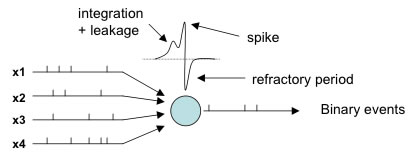
\includegraphics[width=75mm,scale=0.7]{spiking_neuron.jpg}
\caption{Спайковый нейрон}
\label{spiking_neuron_pic}
\end{figure}\\
\subsection{Модель Integrate-and-fire}
\indent Самая простая спайковая модель, основанная на RC цепи, записывается в виде дифференциального уравнения
   \begin{equation}\label{eq:iaf}
   \tau_{m}\frac{du}{dt} =-u+R I(t),
   \end{equation}
при $u \geq \vartheta$ потенциал мембраны сбрасывается и на $\tau_{ref}$ держится в сброшенном состоянии
   \begin{equation}\label{eq:iaf_reset}
   u \leftarrow u_{r} \mbox{ в течении }\tau_{ref}, 
   \end{equation}
   где $\vartheta$ - порог напряжения, временная константа мембраны $\tau_{m}=RC$, $R$ и $C$ - сопротивление и ёмкость RC-цепи соответственно, $\tau_{ref}$ - рефракторное время, $I(t)$ - приложенный ток извне, $u_{r}$ - константа описывающая потенциал мембраны покоя нейрона.\\
   \indent Пример работы такого нейрона можно посмотреть на рис.\ref{iaf_neuron_pic}.\\
\begin{figure}[ht]
\centering
\captionsetup{justification=centering,margin=1cm}
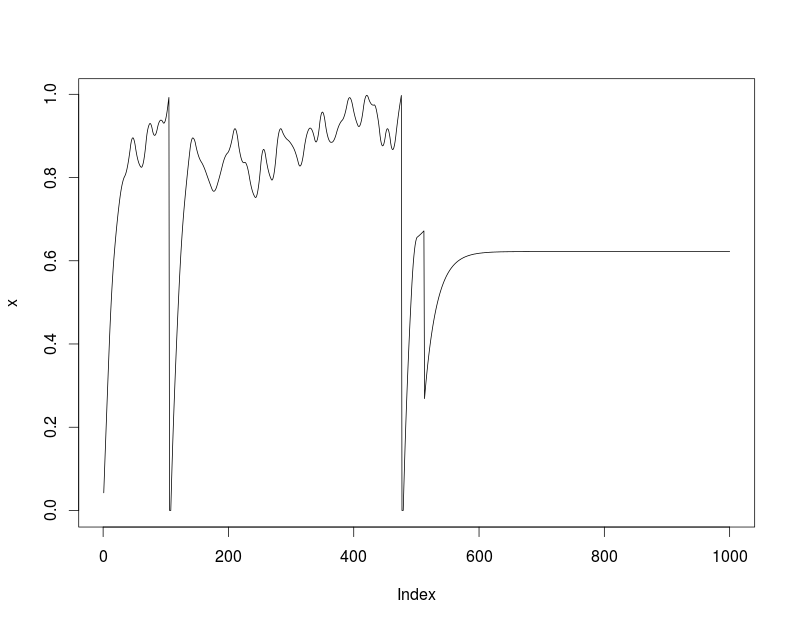
\includegraphics[width=120mm,scale=1]{iaf_profile.png}
\caption{Напряжение на мембране IaF, при $u_{r} = 0, \vartheta = 1, \tau_{ref} = 2$ мс, $\tau_{m} = 20$ мс}
\label{iaf_neuron_pic}
\end{figure}\\
\FloatBarrier

\section{Cтатичный синапс}
\indent При формировании спайковых нейронных сетей наиболее натуральный способ передачи сигнала от одного нейрона к другому -- через синаптические связи. Биологически адекватной моделью является модель синапса с быстрым экспоненциальным ростом (1-5 мс), а затем медленным (10-100 мс) угасанием. Такая динамика хорошо описывает высвобождение нейромедиаторов в синаптическую щель, проведение импульса на постсинаптическую мембрану, а затем медленное угасание этого импульса \cite{wiki:epsp}. См. рис. \ref{synapse_pic}
\begin{figure}[ht]
\centering
\captionsetup{justification=centering,margin=1cm}
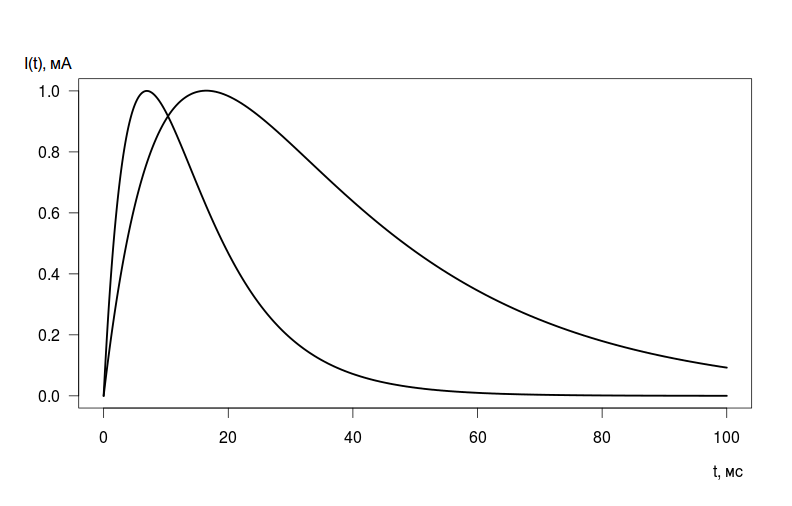
\includegraphics[width=120mm,scale=1]{syn_exp.png}
\caption{Динамика синапса}
\label{synapse_pic}
\end{figure}\\
\FloatBarrier


\section{Гедонистический синапс}
\indent В работе Seung\cite{seung2003learning} была представлена модель синапса в разрезе теории обучения с подкреплением -- предполагается, что активность синапса напрямую альтерируется размером награды в системе. Теоретическая модель в своей основе, модель не претендует на серьезные биологические обоснования, но тем не менее модель отражает некоторые известные биологические феномены, например такой как выработка оперантного условного рефлекса.\\
\indent Модель гедонистического синапса устроена так, что синапс может находится в двух состояниях: состояние доступности (\textit{A}), состояние рефракторности (\textit{R}). Когда синапс доступен вероятность того, что синапс высвободит нейромедиаторы и проведёт входной импульс задается softmax формулой:
\begin{equation*}
p = \frac{1}{1 + e^{-q-c}},
\end{equation*}
которая является функцией от параметра натренированности синапса $q$ и параметра $c$, который задает динамику кальция в синапсе. Чем больше значение этих двух параметров, тем выше вероятность проведения спайка.\\
\indent Параметры $q$ и $c$ изменяются во времени и имеют разную динамику. Параметр $q$ изменяется на большом промежутке времени, обучение нейрона охрактеризовано именно этим параметром, этот параметр можно описать как веротностный вес синапса. Параметр $c$ задает динамику на небольшом промежутке (около 0.5 с) и является как бы катализатором спайков синапса -- при большом количестве спайков на входе синапса, синапс увеличивает вероятность своего спайка.\\
\indent При каждом спайке синапса переменная $c$ увеличивается на небольшую константу $\Delta c$, после чего $c$ угасает с динамикой описываемой уравнением:
\begin{equation}\label{eq:decay}
\frac{dc}{dt} = - c / \tau_{c},
\end{equation} 
где $\tau_{c}$ временная константа порядка 500 мс.\\
\indent Так же, при каждом спайке синапса, спайк оставлет т.н. след на синапсе, который угасает в заданном порядке (от 20 мс, до 1 с). Этот элемент является ключевым в обучении синапса следовать награде. При спайке переменная $e$ увеличивается на значение $\Delta e$:
\begin{equation}\label{eq:delta_e}
\Delta e = \begin{cases} 1-p, \quad \text{при выбросе нейромедиатора} \\ -p, \quad \text{при неудаче выброса} \\ \end{cases},
\end{equation}
угасание описывается аналогичной динамикой, как в динамике кальция \ref{eq:decay}, только с временной константой $\tau _e$\\
\indent При включении системы награды и наказания в данную модель, где уровень награды описывается переменной $R$, динамику вероятностного веса синапса $q$, можно описать уравнением
\begin{equation*}
\frac{dq}{dt} = \eta R(t) e(t)
\end{equation*}
где $\eta$ маленький коэффициент обучения.\\
\indent След активности синапса $e$ играет роль памяти в системе, если синапс произвёл определенную активность и получил награду в ближайшее время (зависит от $\tau_e$), то вероятность выброса нейромедиатора напрямую альтерируется корреляцией $e$ и $R$. Причём, если синапс имеет слабый вероятностный вес $q$, он провалил провести потенциал (т.е. монетка подрошенная для семплирования вероятности $p$ показала неудачу) и получил награду, то $q$ в целом уменьшается на значения $-p$ (см. \ref{eq:delta_e}). В случае же когда синапс выпустил нейромедиатор и награда пришла, но веротность увеличивается на значение $1-p$.
\section{Исследование классификатора}
*в разработке*
\bibliography{refs}{}
\bibliographystyle{unsrt}

\end{document}
